\documentclass[11pt,a4]{jarticle}
\usepackage[top=25truemm,bottom=30truemm,left=20truemm,right=20truemm]{geometry}
\usepackage{graphicx}
\usepackage{comment}
\begin{document}

\title{光波}
\author{レポート提出者: 平松信義; 共同実験者: 森本颯太.}
\date{実験日: 平成29年7月10日、11日\\レポート提出日: 平成29年7月28日}
\maketitle
\tableofcontents

\section{実験の目的}
光学現象は一般に本実験では回折現象と偏光に関して様々な測定を行い、光学一般への理解を深めることを目的とした。

\section{実験方法}
\subsection{回折}
はじめに単スリットを通過したレーザー光をスクリーンに映し、回折現象を観察した。光学系の模式図を図\ref{fig:single_slit}に示した。
スクリーンと単スリットの距離と単スリットのスリット幅をそれぞれ変化させたときの回折パターンを、
CCDカメラを用いて読み取った。光源にはCO$_2$レーザー (波長632.8 nm) を用いた。
\begin{figure}[htbp]
   \begin{center}
    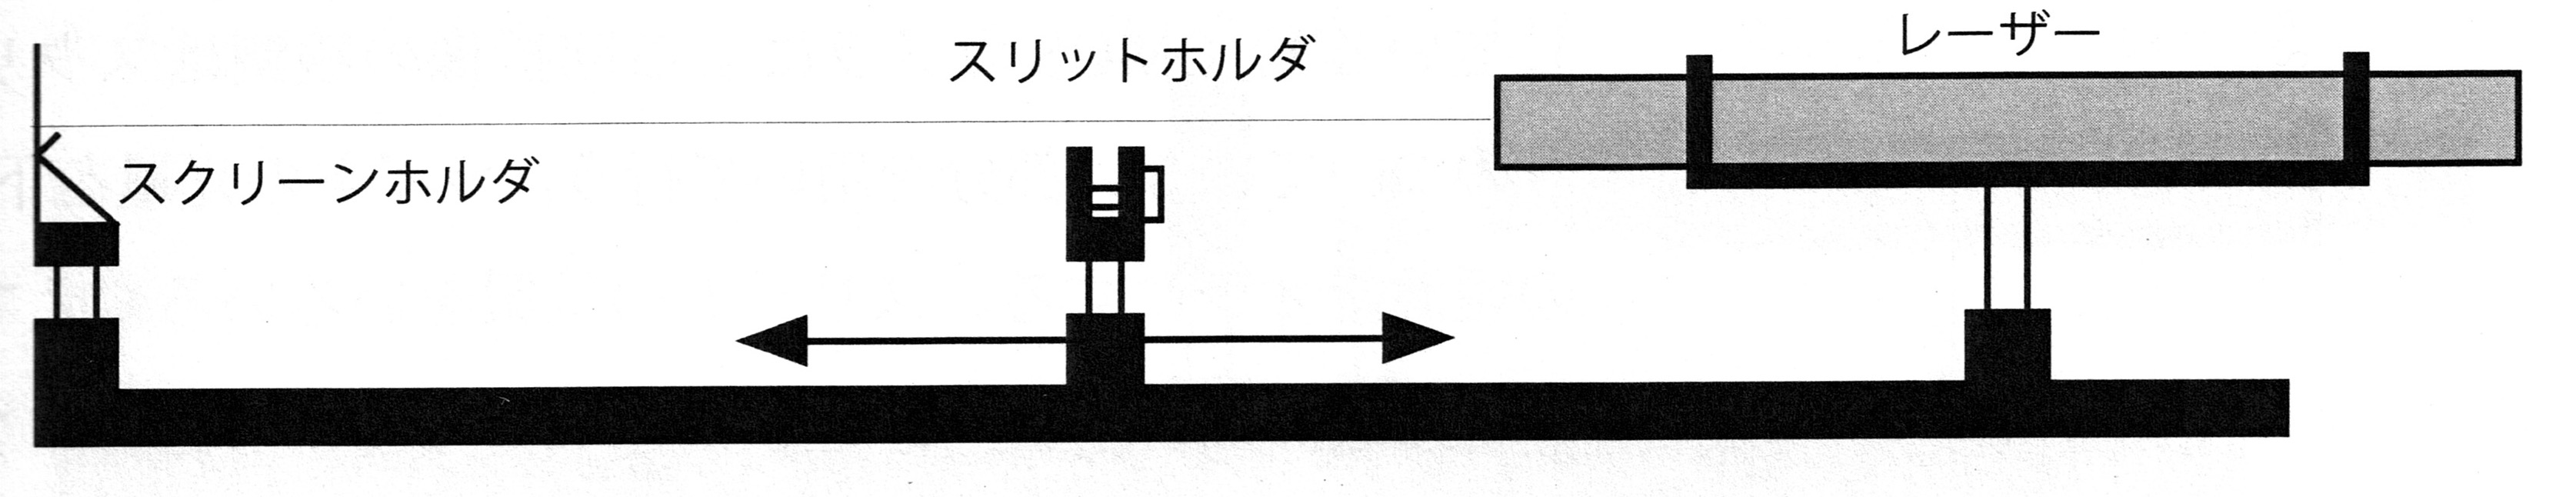
\includegraphics[width=0.9\hsize]{./single_slit.eps}
    \caption{単スリットを通過した光の回折現象の測定系}
     \label{fig:single_slit}
   \end{center}
\end{figure}

任意の点における電磁波の振幅は離れた点から来た球面波の重なりで表すことができるというフレネルの原理から、回折パターンはよく説明できる。
さらに、$z$をスクリーンと単スリットの距離、$d$をスリット幅、$\lambda$を波長とすると、以下の条件を満たすときフラウンホーファーの近似を用いて回折パターンが説明できる。
\begin{equation}
\lambda >> d^2 /4z
\label{eq:joken}
\end{equation}
このとき明線間隔$x$は以下で与えられる。
\begin{equation}
x =  \frac{\lambda z}{d} \alpha
\label{eq:meisen}
\end{equation}
ここで$\alpha$は光軸に対するスクリーンの傾きを補正する係数であり、本実験では$\alpha=\sqrt{2}$程度にとった。

次に、スリットとスクリーンの間に新たに凸レンズを入れた光学系を図\ref{fig:Fourier}のように構成した。
\begin{figure}[htbp]
   \begin{center}
    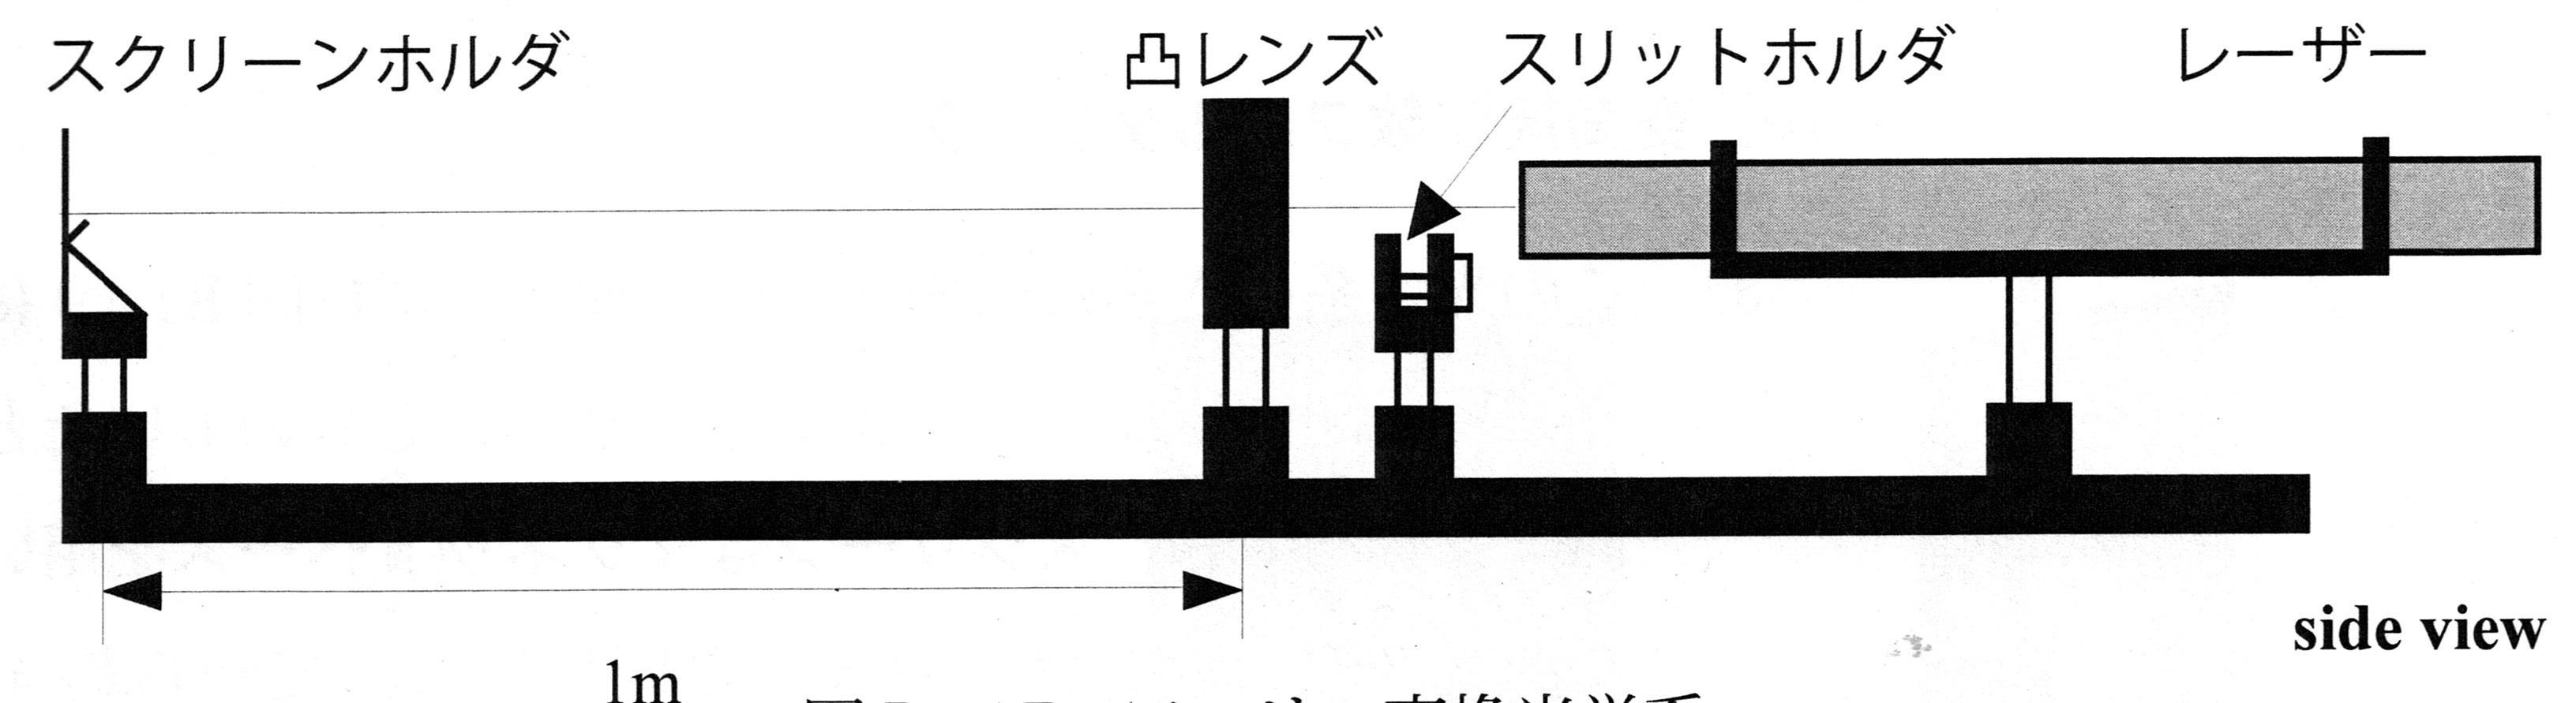
\includegraphics[width=0.9\hsize]{./Fourier.eps}
    \caption{空間周波数フィルタリング光学系}
     \label{fig:Fourier}
   \end{center}
\end{figure}
このとき凸レンズの焦点がスクリーン上に来るように光学系を調整した。

さらに図\ref{fig:koshi}に示すような回折格子A、B、Cにレーザー光を入射してその回折を観察した。回折格子Cでは横縞の間隔に比べ、縦縞の間隔が広い。
\begin{figure}[htbp]
   \begin{center}
    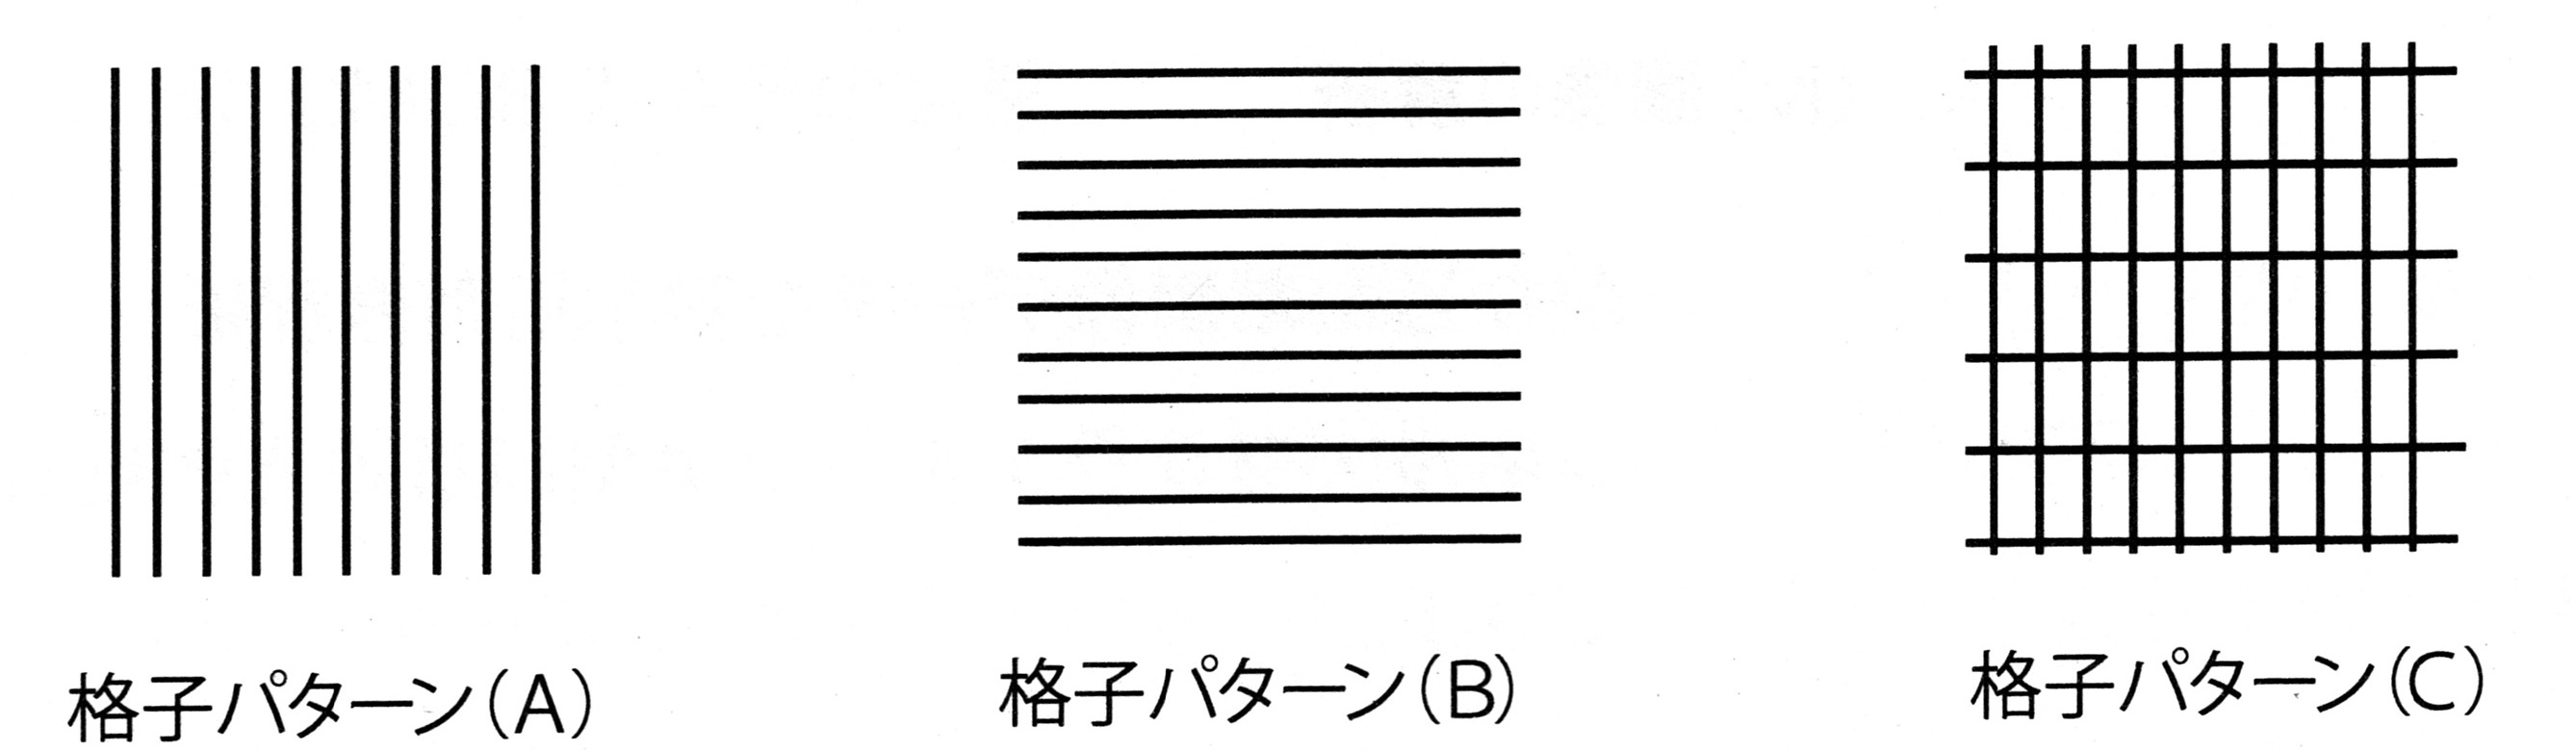
\includegraphics[width=0.9\hsize]{./koshi.eps}
    \caption{格子パターン}
     \label{fig:koshi}
   \end{center}
\end{figure}

さらに"E"文字型のスリットと"C"文字型のスリットの回折模様を観察し、文字Eと文字Cを空間フーリエ変換したものと比較した。"E"文字型のスリットに関しては回折光の一部を取り出して、それを再び結像することで、元の文字Eを再現した。

次に図\ref{fig:koshi_AB}に示すような回折格子について、回折パターンから縦方向のモードと横方向のモードをそれぞれ抜き出して逆に結像して、その逆像を観察した。
\begin{figure}[htbp]
   \begin{center}
    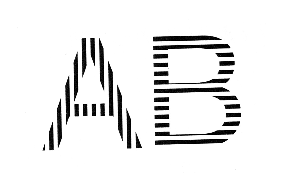
\includegraphics[width=0.4\hsize]{./koshi_AB.eps}
    \caption{格子パターン2}
     \label{fig:koshi_AB}
   \end{center}
\end{figure}


\subsection{偏光}
まず波長板で偏光がどのように変化するか実験で確かめた。
光学系を図\ref{fig:polarization}に示す。
2つの偏光板の間に波長板を挿入する。一つ目の偏光板(光源側)の光学軸に対してもう一方の偏光板の光学軸を変化させ、透過する光量を測定した。
\begin{figure}[htbp]
   \begin{center}
    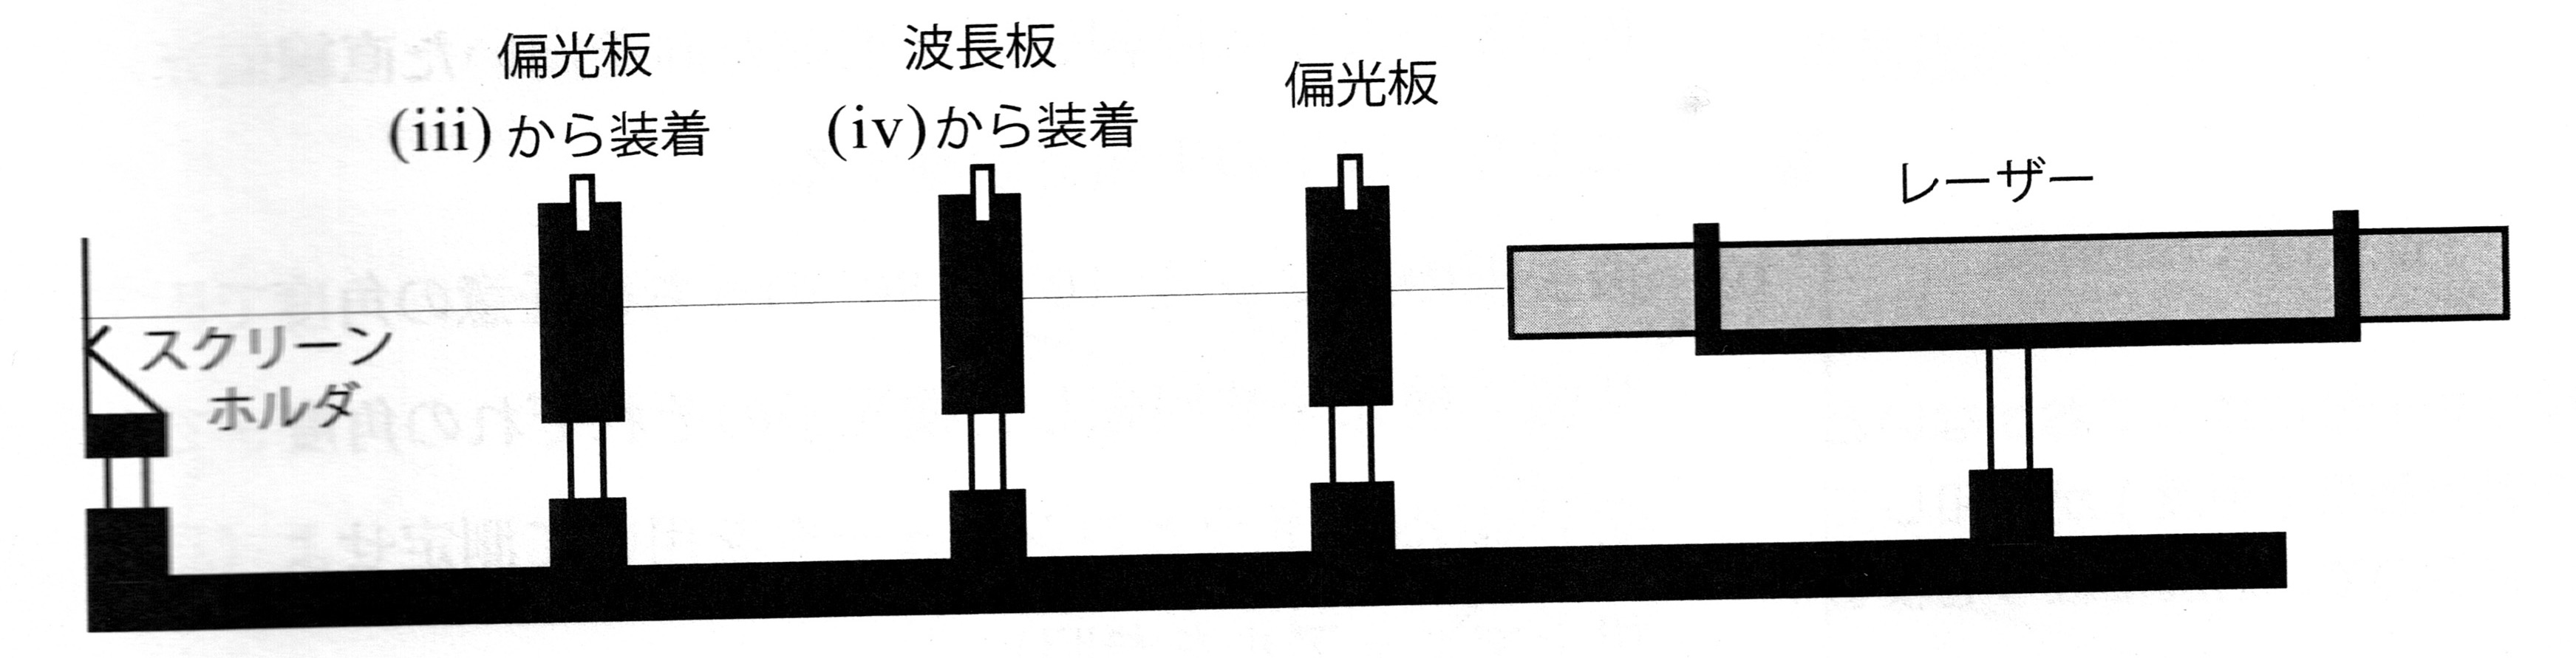
\includegraphics[width=0.9\hsize]{./polarization.eps}
    \caption{}
     \label{fig:polarization}
   \end{center}
\end{figure}

次に偏光顕微鏡を用いて球晶を観察した。図\ref{fig:henko_kenbikyo}に模式図を示す。直線偏光が資料に入射されて透過した光のうち入射光と直交する成分を顕微鏡で検出する。
\begin{figure}[htbp]
   \begin{center}
    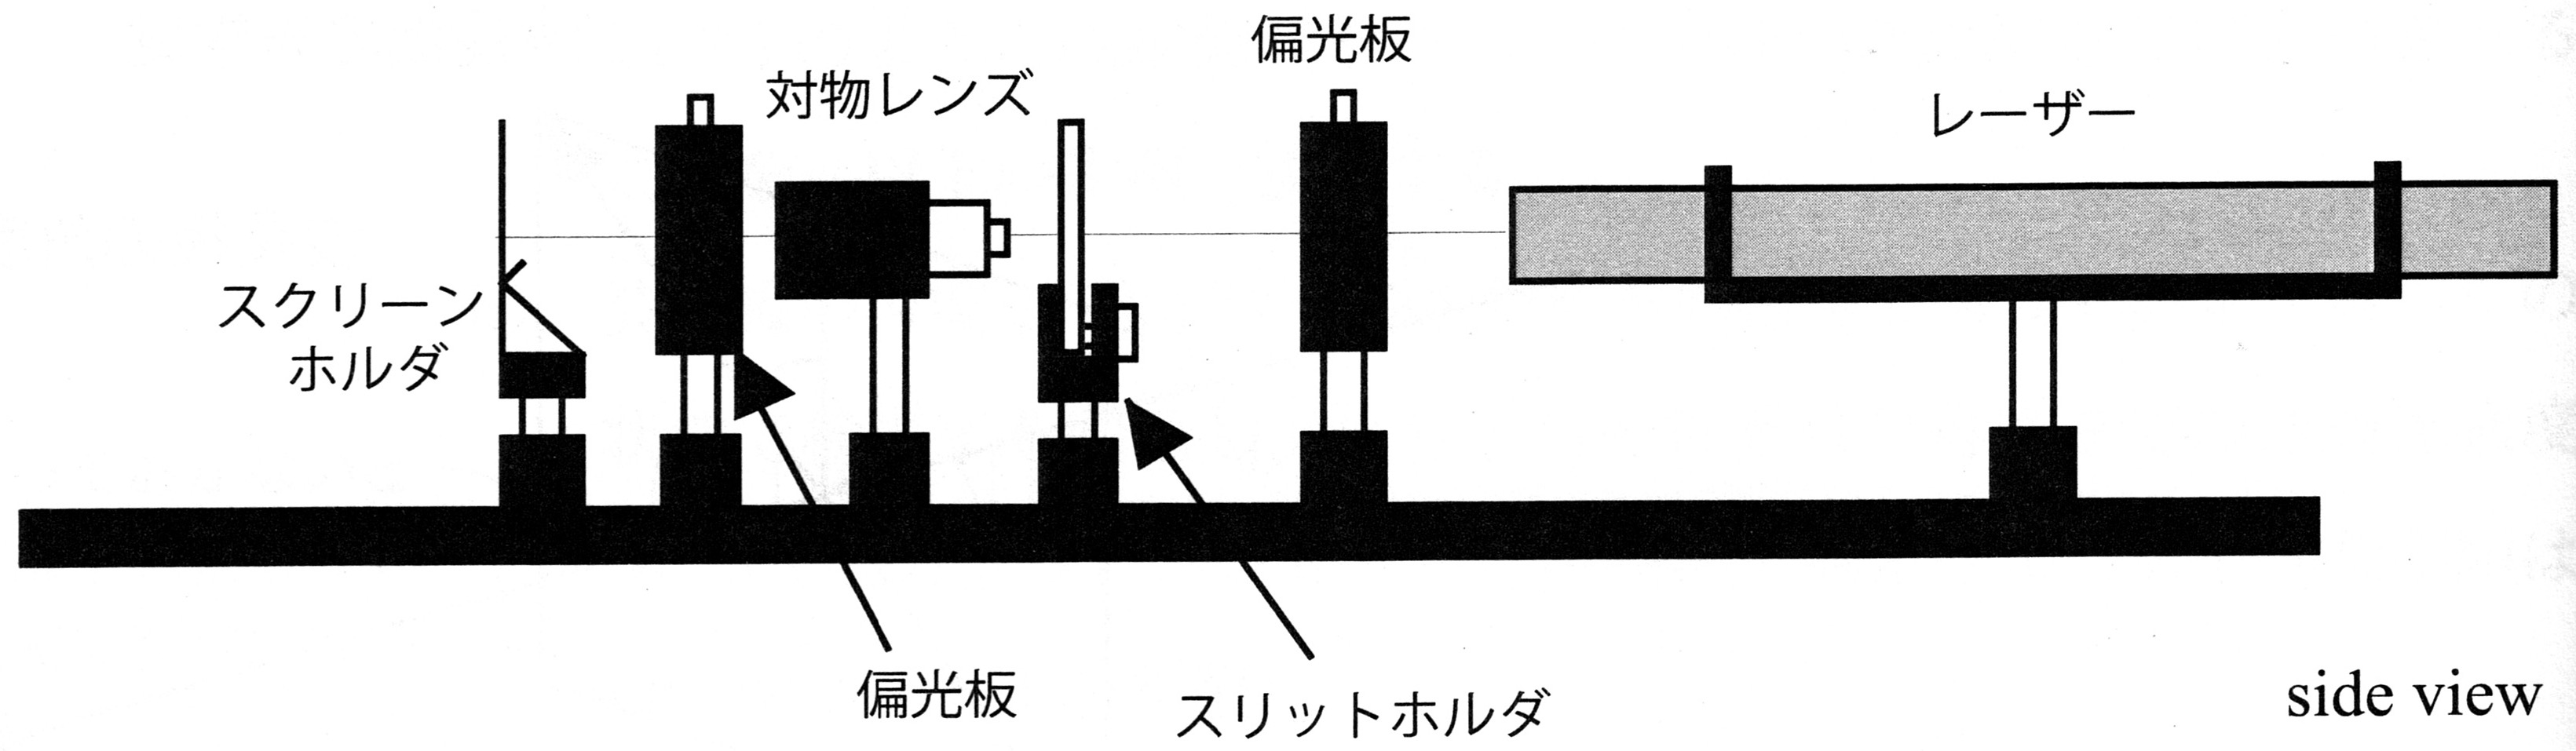
\includegraphics[width=0.9\hsize]{./henko_kenbikyo.eps}
    \caption{}
     \label{fig:henko_kenbikyo}
   \end{center}
\end{figure}

\section{実験結果}
\subsection{回折}
幅2.48mmの単スリットを用いて、スクリーンと単スリットの距離を50cm、75cm、100cmとしたとき観測した回折パターンのプロファイルをそれぞれ図\ref{fig:2480um_50cm}、\ref{fig:2480um_75cm}、\ref{fig:2480um_100cm}に示した。特定の位置に局在したフレネル型の回折パターンが観測され、スクリーンと単スリットの距離を変えても回折パターンに大きな違いは見られなかった。
\begin{figure}[htbp]
   \begin{center}
    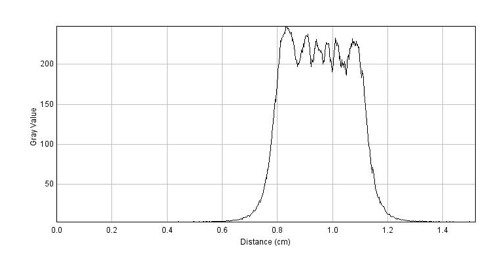
\includegraphics[width=0.5\hsize]{./2480um_50cm_profile.eps}
    \caption{スリット幅 2.48mm, スクリーンと単スリットの距離50cm }
     \label{fig:2480um_50cm}
   \end{center}
\end{figure}\begin{figure}[htbp]
   \begin{center}
    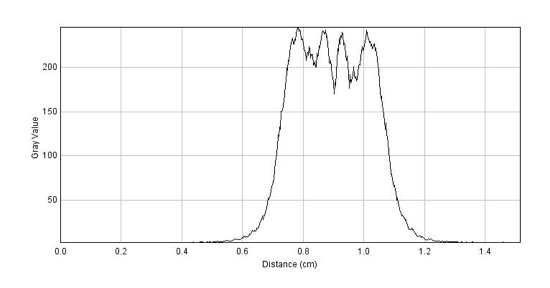
\includegraphics[width=0.5\hsize]{./2480um_75cm_profile.eps}
    \caption{スリット幅 2.48 mm, スクリーンと単スリットの距離75 cm}
     \label{fig:2480um_75cm}
   \end{center}
\end{figure}
\begin{figure}[htbp]
   \begin{center}
    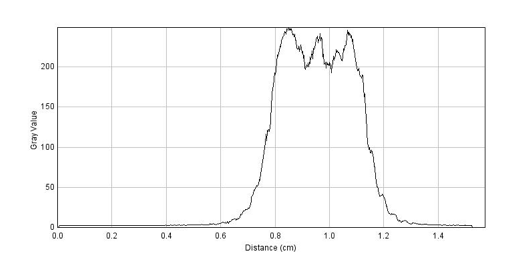
\includegraphics[width=0.5\hsize]{./2480um_100cm_profile.eps}
    \caption{スリット幅 2.48 mm, スクリーンと単スリットの距離50 cm}
     \label{fig:2480um_100cm}
   \end{center}
\end{figure}


次に幅0.26mmの単スリットを用いて、スクリーンと単スリットの距離が25cm、50cm、75cm、100cmのとき観測した回折パターンのプロファイルをそれぞれ図\ref{fig:260um_25cm}、\ref{fig:260um_50cm}、\ref{fig:260um_75cm}、\ref{fig:260um_100cm}に示した。条件$\lambda >> d^2 /4z$を満たす領域に特有の、幅が広くて回折縞をもつ回折パターンが観測された(フラウンホーファー型)。
観測した回折パターンから求めた明線間隔と式\ref{eq:meisen}から計算で求めた明線間隔を表\ref{tab:260um}にそれぞれ示した。高い精度での一致が見られる。

\begin{figure}[htbp]
   \begin{center}
    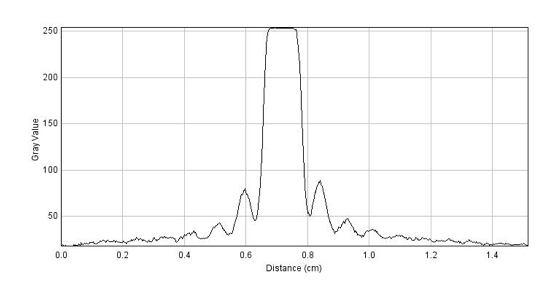
\includegraphics[width=0.48\hsize]{./260um_25cm_profile.eps}
    \caption{スリット幅 0.26 mm, スクリーンと単スリットの距離25 cm}
     \label{fig:260um_25cm}
   \end{center}
\end{figure}
\begin{figure}[htbp]
   \begin{center}
    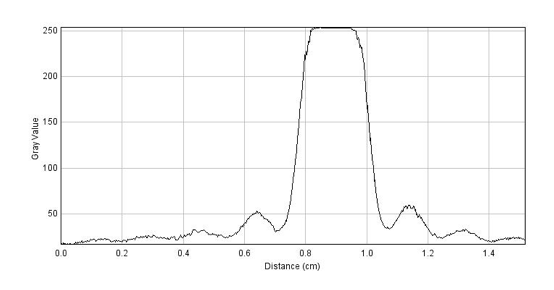
\includegraphics[width=0.48\hsize]{./260um_50cm_profile.eps}
    \caption{スリット幅 0.26 mm, スクリーンと単スリットの距離50 cm}
     \label{fig:260um_50cm}
   \end{center}
\end{figure}\begin{figure}[htbp]
   \begin{center}
    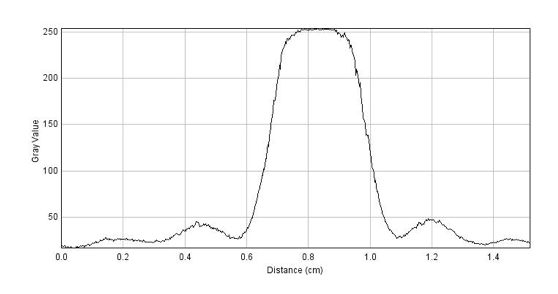
\includegraphics[width=0.48\hsize]{./260um_75cm_profile.eps}
    \caption{スリット幅 0.26 mm, スクリーンと単スリットの距離75 cm}
     \label{fig:260um_75cm}
   \end{center}
\end{figure}\begin{figure}[htbp]
   \begin{center}
    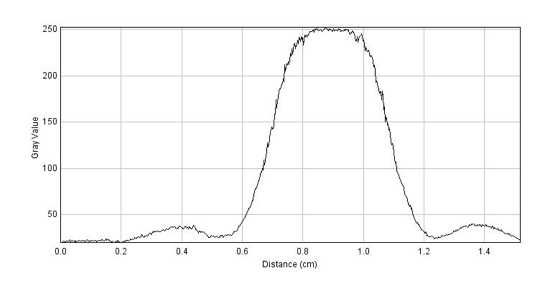
\includegraphics[width=0.48\hsize]{./260um_100cm_profile.eps}
    \caption{スリット幅 0.26 mm, スクリーンと単スリットの距離100 cm}
     \label{fig:260um_100cm}
   \end{center}
\end{figure}

\begin{table}[htbp]
   \begin{center}
  \begin{tabular}{c|cccc}
     スクリーンと単スリットの距離 (cm) & 25 & 50 & 75 & 100 \\ \hline
    明線間隔の実験値 (cm) & 0.08 & 0.17 & 0.29 & 0.37\\
    明線間隔の計算値 (cm) & 0.086 & 0.172 & 0.268 & 0.344
  \end{tabular}
  \label{tab:260um}
     \end{center}
       \caption{明線間隔}
\end{table}

図格子A、B、Cの回折パターンを示した。
縦縞が入った回折格子Aは横方向の回折パターンが観測され、横縞が入った回折格子Bは縦方向の回折パターンが観測された。縦縞と横縞が両方入った回折格子Cでは横方向と縦方向両方の2次元の回折パターンが観測され、縦方向のパターンはが横方向に比べ密に詰まっていることが分かる。
\begin{figure}[htbp]
 \begin{minipage}{0.33\hsize}
   \begin{center}
    
\includegraphics[width=0.9\hsize]{./TypeA.eps}
    \caption{格子パターン(A)}
     \label{fig:TypeA}
   \end{center}
 \end{minipage}
 \begin{minipage}{0.33\hsize}
   \begin{center}
    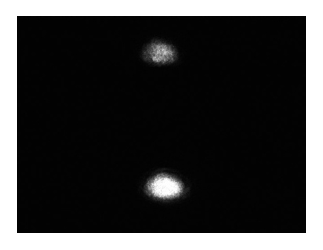
\includegraphics[width=0.9\hsize]{./TypeB.eps}
    \caption{格子パターン(B)}
     \label{fig:TypeB}
   \end{center}
 \end{minipage}
  \begin{minipage}{0.33\hsize}
   \begin{center}
    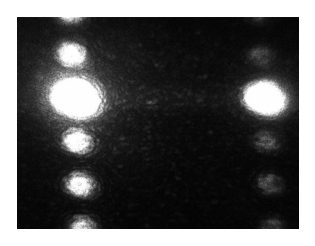
\includegraphics[width=0.9\hsize]{./TypeC.eps}
    \caption{格子パターン(C)}
     \label{fig:TypeC}
   \end{center}
 \end{minipage}
\end{figure}

図\ref{fig:E_exp}と図\ref{fig:C_exp}に"E"文字型スリットと”C”文字型スリットの回折パターンをそれぞれ示した。
また図\ref{fig:E_comp}と\ref{fig:C_comp}に文字Eと文字Cをそれぞれ空間フーリエ変換した結果を示した。
それぞれの文字に対して、回折パターンと空間フーリエ変換が対応していることが分かる。
例えば、文字Eに関しては同様の十字の模様が回折パターンと空間フーリエ変換で見て取れる。
\begin{figure}[htbp]
 \begin{minipage}{0.55\hsize}
   \begin{center}
    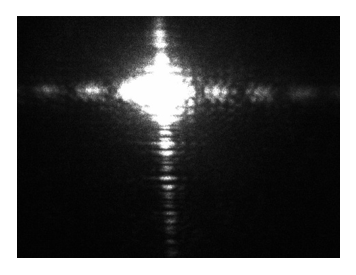
\includegraphics[width=0.9\hsize]{./E_exp.eps}
    \caption{"E"文字型スリットの回折パターン}
     \label{fig:E_exp}
   \end{center}
 \end{minipage}
 \begin{minipage}{0.45\hsize}
   \begin{center}
    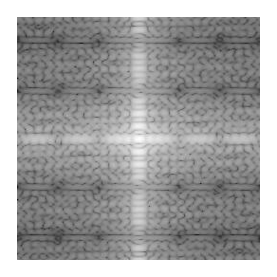
\includegraphics[width=0.9\hsize]{./E_comp.eps}
    \caption{"E"文字型スリットの空間フーリエ変換}
     \label{fig:E_comp}
   \end{center}
 \end{minipage}
\end{figure}

\begin{figure}[htbp]
 \begin{minipage}{0.55\hsize}
   \begin{center}
    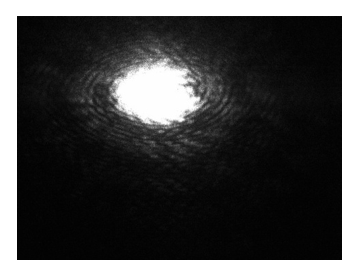
\includegraphics[width=0.9\hsize]{./C_exp.eps}
    \caption{"C"文字型スリットの回折パターン}
     \label{fig:C_exp}
   \end{center}
 \end{minipage}
 \begin{minipage}{0.45\hsize}
   \begin{center}
    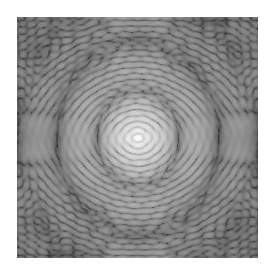
\includegraphics[width=0.9\hsize]{./C_comp.eps}
    \caption{"C"文字型スリットの空間フーリエ変換}
     \label{fig:C_comp}
   \end{center}
 \end{minipage}
\end{figure}

図\ref{fig:E_tate1_exp}と\ref{fig:E_tate1_comp}に、E文字スリットの縦方向の第一モードのみの、逆像とフーリエ逆変換を示した。どちらもEの横線だけが再現されていることが分かる。
図\ref{fig:E_yoko1_exp}と\ref{fig:E_yoko1_comp}に、E文字スリットの横方向の第一モードのみの、逆像とフーリエ逆変換を示した。どちらも縦の線が再現されていることが分かる。
\begin{figure}[htbp]
 \begin{minipage}{0.55\hsize}
   \begin{center}
    
\includegraphics[width=0.9\hsize]{./E_tate1_exp.eps}
    \caption{"E"の縦第一モードの逆像}
     \label{fig:E_tate1_exp}
   \end{center}
 \end{minipage}
 \begin{minipage}{0.45\hsize}
   \begin{center}
    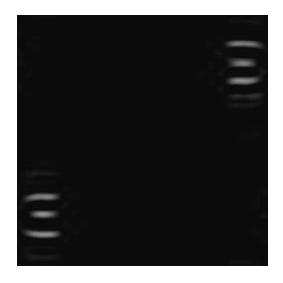
\includegraphics[width=0.9\hsize]{./E_tate1_comp.eps}
    \caption{"E"の縦第一モードの逆変換}
     \label{fig:E_tate1_comp}
   \end{center}
 \end{minipage}
\end{figure}

\begin{figure}[htbp]
 \begin{minipage}{0.55\hsize}
   \begin{center}
    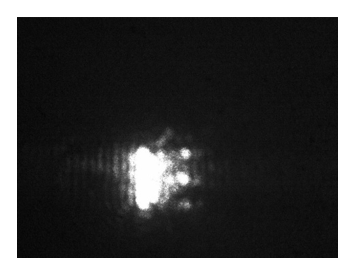
\includegraphics[width=0.9\hsize]{./E_yoko1_exp.eps}
    \caption{"E"の横第一モードの逆像}
     \label{fig:E_yoko1_exp}
   \end{center}
 \end{minipage}
 \begin{minipage}{0.45\hsize}
   \begin{center}
    
\includegraphics[width=0.9\hsize]{./E_yoko1_comp.eps}
    \caption{"E"の横第一モードの逆変換}
     \label{fig:E_yoko1_comp}
   \end{center}
 \end{minipage}
\end{figure}

図\ref{fig:koshi_AB}に示すような格子について、縦モードと横モードを取り出して観察した。
縦モードと横モードを分離しない場合の逆像を図\ref{fig:AB}に示した。これは元の像と一致する。ただし上下と左右が反転している。
横モードのみを抜き出した場合の逆像を図\ref{fig:A}に示した。このとき文字Aだけが逆像に現れることが分かる。
縦モードのみを抜き出した場合の逆像を図\ref{fig:B}に示した。このときは逆に文字Bだけが逆像に現れる。
\begin{figure}[htbp]
 \begin{minipage}{0.33\hsize}
   \begin{center}
    
\includegraphics[width=0.9\hsize]{./AB.eps}
    \caption{通常の逆像}
     \label{fig:AB}
   \end{center}
 \end{minipage}
 \begin{minipage}{0.33\hsize}
   \begin{center}
    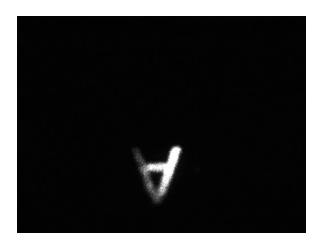
\includegraphics[width=0.9\hsize]{./A.eps}
    \caption{横方向のモードの逆像}
     \label{fig:B}
   \end{center}
 \end{minipage}
  \begin{minipage}{0.33\hsize}
   \begin{center}
    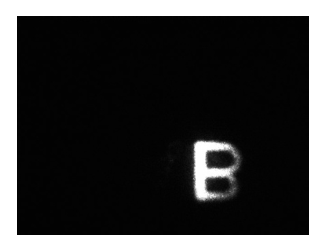
\includegraphics[width=0.9\hsize]{./B.eps}
    \caption{縦方向のモードの逆像}
     \label{fig:B}
   \end{center}
 \end{minipage}
\end{figure}

\subsection{偏光}

一つ目の偏光板(光源側)の光学軸に対して波長板の光学軸を$\psi$度傾けたとき実験を行った。二つ目の偏光板の光学軸は一つ目のものと直交した状態を基準とした。図\ref{fig:HW}に1/2波長板での実験結果を示した。図\ref{fig:HW}に1/4波長板での実験結果を示した。
\begin{figure}[htbp]
   \begin{center}
    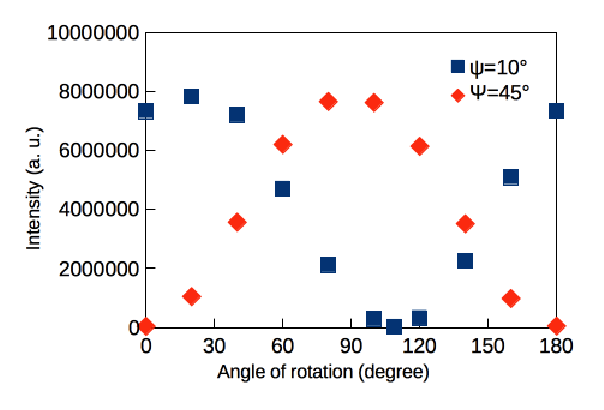
\includegraphics[width=0.9\hsize]{./HW.eps}
    \caption{1/2波長板}
     \label{fig:HW}
   \end{center}
\end{figure}
\begin{figure}[htbp]
   \begin{center}
    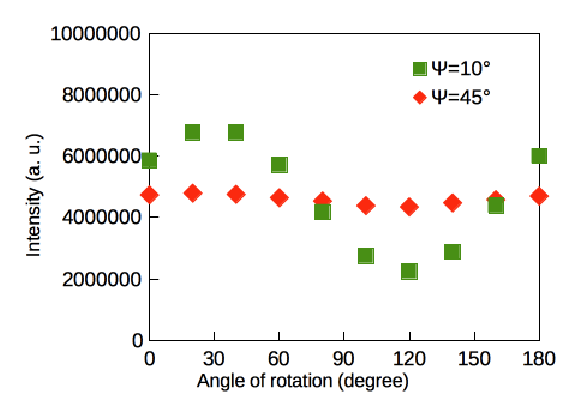
\includegraphics[width=0.9\hsize]{./QW.eps}
    \caption{}
     \label{fig:QW}
   \end{center}
\end{figure}


入射光と検出光が平行な偏光成分を持つとき、入射光に対して検出光が45°傾いた偏光を持っているとき、
入射光と検出光が直交した偏光成分を持つときについて観察し、それぞれ図\ref{fig:conichol}、\ref{fig:45nichol}、\ref{fig:crossnichol1}に示した。図\ref{fig:conichol}と図\ref{fig:45nichol}に比べ図\ref{fig:crossnichol1}では、球晶の外部を透過する光量が大幅に小さくなっている。またそれぞれの条件で球晶の内部を透過する光の偏光が変化していることが見て取れる。

\begin{figure}[htbp]
   \begin{center}
    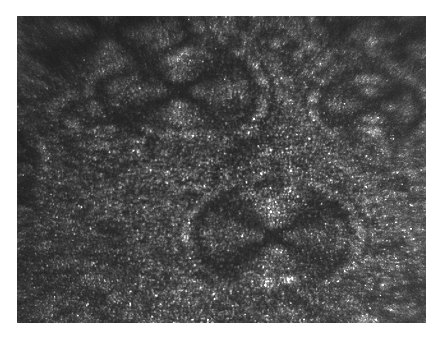
\includegraphics[width=0.7\hsize]{./conichol.eps}
    \caption{}
     \label{fig:conichol}
   \end{center}
\end{figure}
\begin{figure}[htbp]
   \begin{center}
    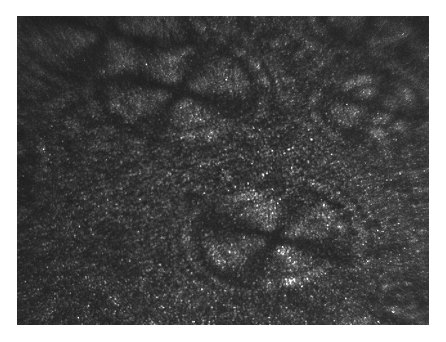
\includegraphics[width=0.7\hsize]{./45nichol.eps}
    \caption{}
     \label{fig:45nichol}
   \end{center}
\end{figure}
\begin{figure}[htbp]
   \begin{center}
    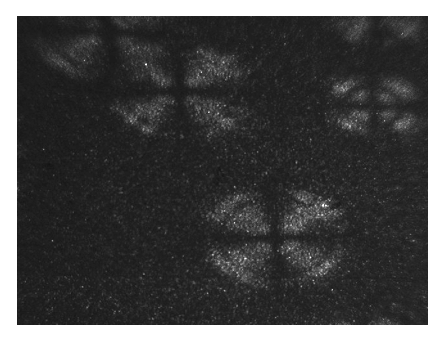
\includegraphics[width=0.7\hsize]{./cross-nichol1.eps}
    \caption{}
     \label{fig:crossnichol1}
   \end{center}
\end{figure}

\section{考察}
\subsection{回折}
フラウンホーファー近似の前提条件\ref{eq:joken}が満たされるかどうか考察する。光源の波長632nmに対して、スリット幅2.48mmのとき$d^2 /4z >1.5 \mu m$であるから条件は満たされない。スリット幅0.26mmのとき$d^2 /4z < 67 nm$であってフラウンホーファー近似が妥当である。

図\ref{fig:Fourier}に示した系では、回折格子の空間フーリエ変換と回折によりできる像は対応している。実際、図3に示した回折格子をそれぞれフーリエ変換(フーリエ展開)すると図14、15、16に示したような離散的なスペクトルが得られる。このとき実格子と逆格子の間隔は逆比例の関係にあることが見て取れる。また図17と図18、図19と図20を比較することで、対応が直接的に分かる。

回折光のモードのから一部のみを取り出したとき、そのモードのに対応して像は一部を再現する。例えば図26で得られた像は横方向のモードを取り出したものに対応し、図27で得られた像は縦方向のモードを取り出したものに対応した。


\subsection{偏光}
1/2波長板を通したあと、どの$\psi$でも強度が0となる検出子の回転角があるから検出光は直線偏光であることが分かる。また偏光軸の回転角(検出光が最大の強度を取る角度)は、$2\psi$に対応している。

1/4波長板で$\psi=45$°としたとき検出光に角度依存性はほとんどなかった。したがって円偏光になっていることが分かる。$\psi=10$°で楕円偏光である。

図32から球晶の内部を透過してきた光の偏光が、入射光から変化していることが分かる。偏光顕微鏡は球晶など波長板や偏光子のような役割を持つ物質の性質を上手く利用して、感度良くそのような物質を検出できることが分かった。

\section{結論}
単スリットの回折実験に関して我々の条件では、スリット幅0.26mmのときフラウンホーファー近似の条件を満たすことを確認し、明線間隔が理論的に予測される値と精度良く一致することを確かめた。また回折格子の空間フーリエ変換と回折によりできる像が対応していることを確かめた。偏光顕微鏡は球晶など波長板や偏光子のような役割を持つ物質の性質を上手く利用して、感度良くそのような物質を検出できることが分かった。

\end{document}